\documentclass[../main.tex]{subfiles}
\begin{document}
\lecture{11}{14.03}{}
\begin{proof}       
    $\begin{aligned}&g(x)\geqslant 0 \; \forall x\geqslant a,\\ &\lim\limits_{x\to +\infty}g(x)=0 \end{aligned}\implies \forall \varepsilon>0 \exists B>0 : \forall x > B \; 0\leqslant g(x)<\frac{\varepsilon}{3M}.$ Берем $\forall b_{1},b_{2}>B\implies \left| \int\limits_{b_{1}        }^{b_{2}} f(x)g(x)dx\right|=\left|\int\limits_{b_{1}}^{b_{2}}g(x)d(F(x))\right| =\left|F(x)g(x)\bigg|_{b_{1}}^{b_{2}}+\int\limits_{b_{1}}^{b_{2}}F(x)(-g'(x))dx\right| =\left| F(b_{2})g(b_{2})-F(b_{1})g(b_{1})+\int\limits_{b_{1}}^{b_{2}}F(x)(-g'(x))dx\right| \\ \leqslant \left|F(b_{2})g(b_{2})\right|+\left|F(b_{1})g(b_{1})\right| +\left|\int\limits_{b_{1}}^{b_{2}} F(x)(-g'(x))dx\right| <\frac{\varepsilon}{3M}\cdot M + \frac{\varepsilon}{3M}\cdot M + M\left|\int\limits_{b_{1}}^{b_{2}} (-g'(x))dx\right|=\frac{2\varepsilon}{3}+\\+M\left|g(b_{1})-g(b_{2})\right|\underset{\text{БОО $b_{2}\geqslant b_{1}$}}{=} \frac{2\varepsilon}{3}+M(\underbrace{g(b_{1})}_{\geqslant 0}-\underbrace{g(b_{2})}_{\geqslant 0})\leqslant \frac{2\varepsilon}{3}+M\cdot \frac{\varepsilon}{3M}=\varepsilon\underset{\text{Кр. Коши}}{\implies} \int\limits_{a    }^{+\infty}f(x)g(x)dx $ сходится.
\end{proof}
$\int\limits_{-\infty   }^{a} $ - формулировка и доказательство - самостоятельно. 

\begin{theorem}
$f(x)$ непрерывна при $x\in [a,b), F(x) - \text{ первообразная к } f(x) \text{ на } [a,b), \exists M>0: |F(x)|\leqslant \\\leqslant M \; \forall x\in[a,b), g(x): \exists g'(x) \; \forall x\in [a,b), g'(x) \text{ непрерывна на } [a,b),g'(x)\leqslant 0 \; \forall x \in[a,b), \lim\limits_{x\to b-0} g(x)=0 \implies\\ \implies \int\limits_{a }^{b    } f(x)g(x)dx $ с особой точкой $b-0$ сходится.
\end{theorem}
\begin{proof}
Самостоятельно.
\end{proof}
$\int\limits_{a }^{b    }  $ с особой точкой $a+0$ - формулировка  и доказательство - самостоятельно. 

\begin{theorem}(признак Абеля)
$f(x):$ 
$
\begin{aligned}
&f(x) \text{ непрерывна при } x\geqslant 0,\\ 
&\int\limits_{a}^{+\infty} f(x)\,dx  \text{ сходится}.
\end{aligned},
$
$g(x):$ 
$
\begin{aligned}
&\exists g'(x) \; \forall x \geqslant a,\\ 
&g'(x) \text{ непрерывна при } x\geqslant a,\\ 
&g'(x)\leqslant 0 \; \forall x\geqslant a,\\
&\exists k>0 : |g(x)|\leqslant k \; \forall x\geqslant a.
\end{aligned}
$ 
$
\implies\int\limits_{a}^{+\infty} f(x)g(x)\,dx \text{ сходится}.
$
\end{theorem}
\begin{proof}
Рассмотрим $F(x) = \int\limits_{a   }^{x}   f(t)dt, \quad \int\limits_{a    }^{+\infty}f(x)dx  $ сходится $\implies \exists \lim\limits_{c  \to +\infty}\int\limits_{a  }^{c    } f(x)dx=A=\lim\limits_{x\to +\infty}F(x)\implies\\ \implies \forall \varepsilon>0 \exists B \geqslant a : \; \forall  x > B \; |F(x)-A|<\frac{\varepsilon}{4k}$
\\ $F(x)$ - первообразная к $f(x)$ на $[a,+\infty)$; Берем $\forall b_{1},b_{2} > B \implies \left| \int\limits_{b_{1}}^{b_{2}}f(x)g(x)dx\right| = \left| \int\limits_{b_{1}}^{b_{2}}g(x)d\left(F(x)-A\right)\right| =\\=\left| (F(x)-A)g(x)\bigg|_{b_{1}}^{b_{2}}+\int\limits_{b_{1}}^{b_{2}} (F(x)-A)(-g'(x))dx\right|  = \left| (F(b_{2})-A)g(b_{2})-(F(b_{1})-A)(g(b_{1}))+\int\limits_{b_{1}}^{b_{2}} (F(x)-A)(-g'(x))dx\right|\leqslant\\\leqslant \left|F(b_{2})-A\right|\cdot|g(b_{2})|+\left|F(b_{1})-A\right|\cdot |g(b_{1})| +\left| \int\limits_{b_{1}}^{b_{2}} (F(x)-A(-g'(x))dx\right| < \frac{\varepsilon}{4k}\cdot k  +\frac{\varepsilon}{4k}\cdot k +\frac{\varepsilon}{4k}\cdot\left|\int\limits_{b_{1}}^{b_{2}}(-g'(x))dx\right| =\\=\frac{\varepsilon}{2}+\frac{\varepsilon}{4k}\left|(g(b_{1})-g(b_{2}))\right| \leqslant \frac{\varepsilon}{2}+\frac{\varepsilon}{4k}(k+k)=\epsilon \underset{\text{Кр. Коши}}{\implies} \int\limits_{a    }^{+\infty}f(x)g(x)dx $ сходится. 
\end{proof}
$\int\limits_{-\infty}^{a} $ - формулировка и доказательство - самостоятельно.
\vspace{0.5cm}
\begin{theorem}
$\begin{aligned}
    &f(x) \text{ непрерывна при } x\in [a,b), \\ 
    &\int\limits_{a  }^{b    } f(x)dx \text{ с особой точкой $b-0$ сходится},\\
\end{aligned},$ $g(x): \begin{aligned}
    &\exists g'(x) \; \forall x\in [a,b),\\
    &g'(x) \text{ непрерывна при } x\in [a,b),\\
    &g'(x)\leqslant 0 \; \forall x\in [a,b),\\
    &\exists k>0: |g(x)|\leqslant k \; \forall x\in [a,b)
\end{aligned} \implies \int\limits_{a   }^{b} f(x)g(x)dx $ с особой точкой $b-0$ сходится.
\end{theorem}
\begin{proof}
Самостоятельно.
\end{proof}
$\int\limits_{a }^{b    } $ с особой точкой $a+0$ - формулировка и доказательство - самостоятельно. 

\subsection{Пример неинтегрируемости модуля интегрируемых в несобственном смысле функций.}
$\int\limits_{1}^{+\infty}\frac{\sin{x}}{x^{p}}dx,\; \int\limits_{1}^{+\infty}\frac{\cos{x}}{x^{p}}dx  $
\\1) $p>1: \quad \left|\frac{\sin{x}}{x^{p}}\right|\leqslant \frac{1}{x^{p}}, \; \left| \frac{\cos{x}}{x^{p}}\right|, \; \int\limits_{1}^{+\infty}\frac{dx}{x^{p}} $ сходится ($p>1$) $\implies \int\limits_{1}^{+\infty}\left| \frac{\sin{x}}{x^{p}}\right| dx  $ и $\int\limits_{1}^{+\infty}\left| \frac{ \cos{x }}{x^{ p} }\right|dx$ сходятся $\implies \int\limits_{1}^{+\infty} \frac{\sin{x}}{x^{p}}dx  $ и $\int\limits_{1}^{+\infty}\frac{\cos{x}}{x^{p}} dx$ сходятся абсолютно. 
\\2) $0<p\leqslant 1: \quad $ Рассмотрим $\int\limits_{1}^{+\infty}\frac{\cos{x}}{x^{p}} dx,$ 
$
\begin{aligned}
&f(x)=\cos{x};\; F(x)=\sin{x}, |F(x)| \leqslant 1\\
&g(x)=\frac{1}{x^{p}}; \; g'(x)=\frac{-p}{x^{p+1}}\in C [1,+\infty),\\
&\frac{-p}{x^{p+1}} \leqslant 0 \; \forall x \geqslant 1,\\
&\lim\limits_{x\to +\infty}\frac{1}{x^{p}}=0
\end{aligned}
\implies \int\limits_{1}^{+\infty}\frac{\cos{x}}{x^{p}}dx $ сходится по признаку Дирихле.
\\ $\left| \frac{\cos{x}}{x^{p}}\right| = \frac{|\cos{x}|}{x^{p}}\geqslant \frac{\cos^{2}{x}}{x^{p}}=\frac{1}{2}\left(\frac{1}{x^{p}}+\frac{\cos{2x}}{x^{p}}\right), \; \int\limits_{1}^{+\infty}\frac{\cos{2x}}{x^{p}}dx$ сходится по Дирихле, но $\int\limits_{1}^{+\infty}\frac{dx}{x^{p}}$ расходится (т.к $p\leqslant 1$) $\implies \int\limits_{1}^{+\infty}\frac{1}{2}\left(\frac{1}{x^{p}}+\frac{\cos{2x}}{x^{p}}\right) dx  $ расходится. $\implies \int\limits_{1}^{+\infty}\left| \frac{\cos{x}}{x^{p}}\right| dx  $ расходится по признаку сравнения $\implies \int\limits_{ 1 }^{+\infty}\frac{\cos{x}}{x^{p}}dx  $ сходится условно. Аналогично $\int\limits_{1  }^{+\infty}\frac{\sin{x}}{x^{p}}dx $ сходится условно. 
\\3) $p\leqslant 0: \quad$ Рассмотрим $\int\limits_{1}^{+\infty}\frac{\sin{x}}{x^{p}}dx.$ Докажем расходимость. 
\\Отрицание критерия Коши: $\int\limits_{1}^{+\infty}\frac{\sin{x}}{x^{p}}dx $ расходится $\Leftrightarrow \exists \varepsilon> 0 : \forall B\geqslant a \; \exists b_{1},b_{2} > B : \left| \int\limits_{b_{1}}^{b_{2}} \frac{\sin{x}}{x^{p}}dx\right|\geqslant \varepsilon$ (?)
\\$\varepsilon=2,$ берем $\forall B\geqslant a\implies \exists b_{1}=2k\pi>B,\exists b_{2} = 2k\pi+\pi > b_{1}>B, k\in\N \; \left| \int\limits_{b_{1}}^{b_{2}}\frac{\sin{x}}{x^{p}}dx\right| = \left| \int\limits_{2k\pi}^{2k\pi+\pi} \frac{\sin{x}}{x^{p}}dx\right|=\int\limits_{2k\pi}^{2k\pi+\pi}\frac{\sin{x}}{x^{p}}dx\underset{\frac{1}{x^{p}}\geqslant 1 \forall x\geqslant 1}{\geqslant}  \int\limits_{2k\pi}^{2k\pi+\pi}\sin{x}dx=2=\varepsilon \implies \int\limits_{1}^{+\infty}\frac{\sin{x}}{x^{p}}dx  $ расходится. Аналогично $\int\limits_{1}^{+\infty}\frac{\cos{x}}{x^{p}}dx$ расходится.
\\Итого: $\int\limits_{1}^{+\infty}\frac{\sin{x}}{x^{p}}dx, \int\limits_{1}^{+\infty}\frac{\cos{x}}{x^{p}} dx $ сходятся абсолютно при $p>1$, сходятся условно при $p\in(0;1]$, расходятся при $p\leqslant 0$.  

\section{Главное значение в смысле Коши несобственных интегралов первого и второго рода и его связь с величиной соответствующего несобственного интеграла.}
\begin{definition}
Пусть $f(x)$ интегрируема в собственном смысле на $\forall[a,b]\subset (-\infty,+\infty)$. Главным значением $\int\limits_{-\infty }^{+\infty}f(x)dx $  в смысле Коши называется число равное $\lim\limits_{R\to +\infty}\int\limits_{-R}^{R} f(x)dx $ (если он существует). Обозначение: $v.p.\int\limits_{-\infty    }^{+\infty  } f(x)dx$ (Valeur Principale, фр).
\end{definition}

\begin{theorem}
Если $\int\limits_{-\infty  }^{+\infty  } f(x)dx$ сходится по Риману, то он сходится и по Коши, причем к той же величине $\left(v.p. \int\limits_{-\infty   }^{+\infty}f(x)=\int\limits_{-\infty    }^{+\infty  } f(x)dx \right)$ 
\end{theorem}
\begin{proof}
$v.p. \int\limits_{-\infty  }^{+\infty}f(x)dx=\lim\limits_{R\to +\infty}\int\limits_{-R}^{R}f(x)dx=\lim\limits_{R\to +\infty}\left[\int\limits_{-R}^{0}f(x)dx +\int\limits_{0}^{R}f(x)dx\right]=\lim\limits_{R\to +\infty}\int\limits_{-R}^{0}f(x)+\\+\lim\limits_{R\to +\infty   } \int\limits_{0}^{R}f(x)dx= \int\limits_{-\infty    }^{0} f(x)dx+\int\limits_{0}^{+\infty   } f(x)dx= \int\limits_{-\infty  }^{+\infty  } f(x)dx  $
\end{proof}
Но не наооборот! 
\begin{proof}
$v.p. \int\limits_{-\infty  }^{+\infty  } \arctan{(x)}dx=\lim\limits_{R\to +\infty}\underbrace{\int\limits_{-R}^{R}\arctan{(x)}dx}_{\substack{\text{интеграл от функции}\\ \text{в симметричных пределах}}}  =0, \text{ но } \int\limits_{-\infty  }^{+\infty  } \arctan{(x)}dx$ расходится, т.к $\int\limits_{0}^{+\infty}\arctan{(x)}dx = \underbrace{\int\limits_{0}^{1}\arctan{(x)}dx}_{\text{собственный}} +\underbrace{\int\limits_{1}^{+\infty}\arctan{(x)}dx}_{\geqslant \frac{\pi}{4}} $
\\ $\int\limits_{1}^{+\infty}\frac{\pi}{4} dx  $ расходится $\implies \int\limits_{0}^{+\infty}\arctan{(x)}dx $ расходится.
\end{proof}


\begin{definition}
Пусть $f(x)$ интегрируема в собственном смысле на $[a,c-\delta]$ и на $[c+\delta,b]\; \forall \delta\in\\\in(a,\min(c-a,b-c)).$ Главным значением $\int\limits_{a  }^{b    } f(x)dx$ в смысле Коши называется число, равное \\$\lim\limits_{\delta\to 0+0}\left[\int\limits_{a}^{c-\delta}f(x)dx +\int\limits_{c+\delta}^{b}f(x)dx\right]$ (если он существует). Обозначение: $v.p.\int\limits_{a}^{b}f(x)dx$.
\end{definition}
\begin{theorem}
Если $\int\limits_{a}^{b}f(x)dx$ сходится по Риману, то он сходится и по Коши, причем к той же величине $\left(v.p.\int\limits_{a}^{b}f(x)dx=\int\limits_{a}^{b}f(x)dx\right)$
\end{theorem}
\begin{proof}
Самостоятельно.
\end{proof}
Но не наоборот! Пусть $a<c<b.$ Рассмотрим $v.p. \int\limits_{a   }^{b    } \frac{dx}{x-c}=\lim\limits_{\delta            \to 0+0}\left[\int\limits_{a  }^{c-\delta}\frac{dx}{x-c}+\int\limits_{c+\delta}^{b}\frac{dx}{x-c}\right]=\\=\lim\limits_{\delta        \to 0+0}\left[\ln{(c-x)}\bigg|_{x=a}^{x=c-\delta} +\ln{(x-c)}\bigg|_{x=c+\delta}^{x=b} \right]= \lim\limits_{\delta\to 0+0} \left[\underbrace{\ln{(\delta)}-\ln{(c-a)}}_{\nexists \lim\limits_{\delta\to 0} }+\underbrace{\ln{(b-c)}-\ln{\delta}}_{\nexists \lim\limits_{\delta\to 0} }\right]=\ln{\left(\frac{b-c}{c-a}\right)}$, но $\int\limits_{a   }^{b    } \frac{dx}{x-c}$ расходится по Риману. 

Если особых точек несколько, то промежуток интегрирования разбиваем так, чтобы особые точки $x_{0}-0$ и $x_{0}+0$ (как и $-\infty$ и $+\infty$) входили попарно. 

Пример: $\int\limits_{-\infty   }^{+\infty  } \frac{dx}{x^{2}-1}$ расходится по Риману.
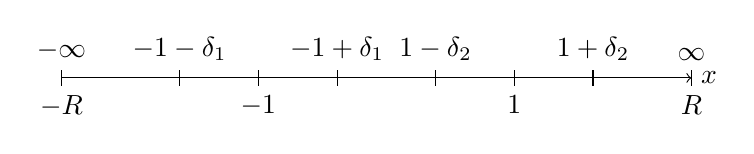
\begin{tikzpicture}[scale=1]
    % Draw the x-axis
    \draw[->] (-4,0) -- (4,0) node[right] {$x$};

    % Draw the points and labels
    \foreach \x/\label in {-4/-\infty, -2.5/-1-\delta_1, -0.5/-1+\delta_1, 0.75/1-\delta_2, 2.75/1+\delta_2, 4/\infty} {
        \draw (\x,0.1) -- (\x,-0.1);
        \node[above] at (\x,0.1) {$\label$};
    }

    % Draw additional points without labels
    \foreach \x in {-4, -1.5, 1.75} {
        \draw (\x,0.1) -- (\x,-0.1);
    }

    % Draw labels for -R and R below the axis
    \node[below] at (-4, -0.1) {$-R$};
    \node[below] at (4, -0.1) {$R$};
    \node[below] at (-1.5, -0.1) {$-1$};
    \node[below] at (1.75, -0.1) {$1$};
\end{tikzpicture}
%$v.p. \int\limits_{-\infty  }^{+\infty  } \frac{dx}{x^{2}-1}=\lim\limits_{\delta_{1}\to 0+0}\left[\int\limits_{-2}^{-1-\delta_{1}}\frac{dx}{x^{2}-1}+\int\limits_{-1+\delta_{1}}^{0}\frac{dx}{x^{2}-1}\right] + \lim\limits_{\delta_{2}\to 0+0}\left[\int\limits_{0}^{1-\delta_{2}} \frac{dx}{x^{2}-1}+\int\limits_{1+\delta_{2}}^{0}\frac{dx}{x^{2}-1}\right] +\lim\limits_{R\to +\infty}\left[ \int\limits_{2}^{R } \frac{dx}{x^{2}-1} +\int\limits_{-R}^{-2}\frac{dx}{x^{2}-1}\right]= \lim\limits_{\delta_{1}\to 0+0}\left[\frac{1}{2 \ln{\left|\frac{x-1}{x+1}\right|}}\bigg|_{-2}^{-1-\delta_{1}}+\frac{1}{2}\ln{\left|\frac{x-1}{x+1}\right|}\bigg|_{-1+\delta_{1}}^{0}\right] + \lim\limits_{\delta_{2}\to 0+0}\left[\frac{1}{2}\ln{\left|\frac{x-1}{x+1}\right|}\bigg|_{0}^{1-\delta_{2}}   + \frac{1}{2}\ln{\left| \frac{x-1}{x+1}\right|}\bigg|_{1+\delta_{2}}^{2}\right] + \lim\limits_{R\to +\infty}\left[\frac{1}{2} \ln{\left| \frac{x-1}{x+1}\right|}\bigg|_{2}^{R}+\frac{1}{2}\ln{\left|\frac{x-1}{x+1}\right|}\bigg_{-R}^{-2}\right] =\underset{\text{самостоятельно}}{\dots}=0\implies \text{ v. p. } \int\limits_{-\infty   }^{+\infty}\frac{dx}{x^{2}-1}=0$
$v.p. \int\limits_{-\infty  }^{+\infty  } \frac{dx}{x^{2}-1}=\lim\limits_{\delta_{1}\to 0+0}\left[\int\limits_{-2}^{-1-\delta_{1}}\frac{dx}{x^{2}-1}+\int\limits_{-1+\delta_{1}}^{0}\frac{dx}{x^{2}-1}\right] + \lim\limits_{\delta_{2}\to 0+0}\left[\int\limits_{0}^{1-\delta_{2}} \frac{dx}{x^{2}-1}+\int\limits_{1+\delta_{2}}^{2}\frac{dx}{x^{2}-1}\right] +\\+\lim\limits_{R\to +\infty}\left[ \int\limits_{2}^{R } \frac{dx}{x^{2}-1} +\int\limits_{-R}^{-2}\frac{dx}{x^{2}-1}\right]= \lim\limits_{\delta_{1}\to 0+0}\left[\frac{1}{2} \ln{\left|\frac{x-1}{x+1}\right|}\Bigg|_{-2}^{-1-\delta_{1}}+\frac{1}{2}\ln{\left|\frac{x-1}{x+1}\right|}\Bigg|_{-1+\delta_{1}}^{0}\right] +\\+ \lim\limits_{\delta_{2}\to 0+0}\left[\frac{1}{2}\ln{\left|\frac{x-1}{x+1}\right|}\Bigg|_{0}^{1-\delta_{2}}   + \frac{1}{2}\ln{\left| \frac{x-1}{x+1}\right|}\Bigg|_{1+\delta_{2}}^{2}\right] + \lim\limits_{R\to +\infty}\left[\frac{1}{2} \ln{\left| \frac{x-1}{x+1}\right|}\Bigg|_{2}^{R}+\frac{1}{2}\ln{\left|\frac{x-1}{x+1}\right|}\Bigg|_{-R}^{-2}\right] =\underset{\text{самостоятельно}}{\dots}=\\=0\implies \text{ v. p. } \int\limits_{-\infty   }^{+\infty}\frac{dx}{x^{2}-1}=0$





\vspace{1cm}
\begin{flushright}
    \textit{tg: @moksimqa}
\end{flushright}